\documentclass[11pt,a4paper]{article}

\usepackage[margin=2.3cm]{geometry}
\usepackage[T1]{fontenc}
\usepackage{lmodern}
\usepackage{microtype}
\usepackage{amsmath,amssymb}
\usepackage{bm}
\usepackage{xcolor}
\usepackage{tikz}
\usetikzlibrary{arrows.meta,calc,decorations.pathmorphing,decorations.markings,patterns,positioning,shapes.geometric,trees,backgrounds}
\usepackage{pgfplots}
\pgfplotsset{compat=1.17}
\usepackage{algorithm}
\usepackage{algpseudocode}
\usepackage[most]{tcolorbox}
\usepackage{caption}
\usepackage{subcaption}
\usepackage{enumitem}
\usepackage[colorlinks=true,linkcolor=blue!50!black,urlcolor=blue!50!black]{hyperref}

% ------------------------------------------------------------------
% colours used consistently in every figure
% ------------------------------------------------------------------
\definecolor{cPrimary}{HTML}{1F5FBF}   % camera / primary rays
\definecolor{cShadow}{HTML}{5A5A5A}    % shadow rays
\definecolor{cRefl}{HTML}{C0392B}      % reflection rays
\definecolor{cRefr}{HTML}{1E8449}      % refraction rays
\definecolor{cNormal}{HTML}{7D3C98}    % normals
\definecolor{cLight}{HTML}{E5A00D}     % light sources
\definecolor{cGlass}{HTML}{D6EAF8}     % transparent objects
\definecolor{cSolid}{HTML}{D5D8DC}     % opaque objects

\tikzset{
  >={Stealth[length=2.6mm]},
  primary/.style={cPrimary, thick, ->},
  shadowray/.style={cShadow, thick, dashed, ->},
  reflray/.style={cRefl, thick, ->},
  refrray/.style={cRefr, thick, ->},
  normal/.style={cNormal, thick, ->},
  glass/.style={draw=blue!50!black, fill=cGlass},
  solid/.style={draw=black!70, fill=cSolid},
  lamp/.pic={\fill[cLight] (0,0) circle (0.13);
             \foreach \a in {0,45,...,315}
               \draw[cLight, thick] (\a:0.19) -- (\a:0.32);},
  eye/.pic={\fill[black] (0,0) circle (0.07);
            \draw[thick] (0.32,0.2) arc (30:-30:0.4);},
  ground/.style={postaction={decorate},decoration={markings,
     mark=between positions 0.02 and 1 step 0.06 with {\draw[black!60] (0,0) -- ++(-0.12,-0.14);}}},
}

\newtcolorbox{inshort}[1][]{colback=blue!3, colframe=blue!45!black,
  fonttitle=\bfseries, title={In short}, boxrule=0.6pt, arc=2pt, #1}
\newtcolorbox{aside}[1]{colback=black!3, colframe=black!45,
  fonttitle=\bfseries, title={#1}, boxrule=0.5pt, arc=2pt}

\newcommand{\vv}[1]{\mathbf{#1}}
\newcommand{\unit}[1]{\widehat{#1}}
\newcommand{\dotp}[2]{\langle #1, #2\rangle}
\algrenewcommand\algorithmiccomment[1]{\hfill{\color{black!55}\(\triangleright\) #1}}
\algnewcommand\algorithmicforeach{\textbf{for each}}
\algdef{S}[FOR]{ForEach}[1]{\algorithmicforeach\ #1\ \algorithmicdo}

\title{\textbf{How the Freestyle Ray Tracer Works}\\[4pt]
\large A visual walk through primary, shadow, reflected and refracted rays}
\author{}
\date{}

\begin{document}
\maketitle

\begin{abstract}
This tutorial explains, step by step, how the freestyle ray tracer turns a scene
description into an image. It deliberately avoids talking about code and
variable names: every stage is described as geometry and arithmetic, illustrated
with a figure and summarised with a short algorithm. The focus is on the life of
a \emph{ray}: how it is born at the camera, how it finds the surface it hits, how
\emph{shadow rays} decide whether that surface is lit, and how
\emph{reflected} and \emph{refracted} rays carry the picture further. The last
section assembles everything into one complete algorithm.
\end{abstract}

\tableofcontents
\newpage

%===================================================================
\section{The big picture}
%===================================================================

A ray tracer runs the physics of light \emph{backwards}. Rather than following
the billions of photons a lamp emits and hoping a few reach the eye, it starts at
the eye, shoots one ray through every pixel and asks: \emph{what colour of light
arrives along this line?} To answer, it finds the first surface the ray hits and
then shoots more rays from there:

\begin{itemize}[leftmargin=1.4em]
  \item a \textbf{shadow ray} towards each light, to check whether the point is lit;
  \item a \textbf{reflected ray}, if the surface is shiny or transparent;
  \item a \textbf{refracted ray}, if the surface lets light through.
\end{itemize}

The reflected and refracted rays are handled exactly like the original ray, so
the whole process is \emph{recursive}. A depth budget stops it eventually.
Figure~\ref{fig:overview} shows all four kinds of ray at once.

\begin{figure}[h]
\centering
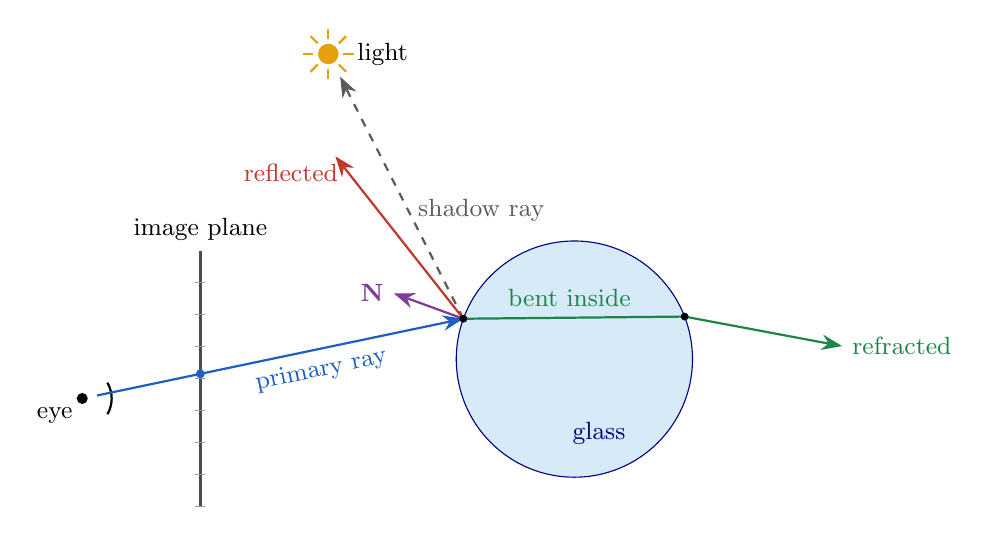
\begin{tikzpicture}[scale=1.25]
  % image plane
  \draw[very thick, black!70] (1.2,-1.1) -- (1.2,1.5) node[above, black] {\small image plane};
  \foreach \y in {-1.1,-0.775,...,1.5} \draw[black!40] (1.15,\y) -- (1.25,\y);
  \fill[cPrimary] (1.2,0.251) circle (0.045);
  % eye
  \pic at (0,0) {eye};
  \node[below left] at (0,0) {\small eye};
  % glass sphere
  \draw[glass] (5,0.4) circle (1.2);
  \node[blue!50!black] at (5.25,-0.35) {\small glass};
  % light
  \pic at (2.5,3.5) {lamp};
  \node[right=7pt] at (2.5,3.5) {\small light};
  % primary
  \draw[primary] (0.15,0.03) -- (3.872,0.810) node[pos=0.6, below, sloped] {\small primary ray};
  % normal
  \draw[normal] (3.872,0.810) -- ++(-0.705,0.257) node[left] {\small $\vv N$};
  % shadow
  \draw[shadowray] (3.872,0.810) -- (2.62,3.27) node[pos=0.45, right] {\small shadow ray};
  % reflected
  \draw[reflray] (3.872,0.810) -- ++(-1.30,1.65) node[pos=0.9, left] {\small reflected};
  % refracted, inside then out
  \draw[cRefr, thick] (3.872,0.810) -- (6.120,0.832);
  \draw[refrray] (6.120,0.832) -- ++(1.6,-0.30) node[right] {\small refracted};
  \fill (3.872,0.810) circle (0.04);
  \fill (6.120,0.832) circle (0.04);
  \node[above] at (4.95,0.83) {\small\color{cRefr} bent inside};
\end{tikzpicture}
\caption{One pixel's story. The primary ray (blue) leaves the eye through a pixel and
hits a glass sphere. From the hit point a shadow ray (dashed) checks the light, a
reflected ray (red) bounces off and a refracted ray (green) bends into the
sphere, bends again on the way out and continues into the scene.}
\label{fig:overview}
\end{figure}

\paragraph{A ray} is a half-line with an origin $\vv o$ and a unit direction $\unit{\vv d}$:
\[
  \vv r(t) = \vv o + t\,\unit{\vv d}, \qquad t > 0 .
\]
Because the direction has unit length, the parameter $t$ is exactly the distance
travelled. ``Nearest hit'' therefore just means ``smallest positive $t$''.

\paragraph{Colours} are 8-bit RGB triples. Every stage below produces a colour,
and colours from different rays are blended with weights between $0$ and $1$.

%===================================================================
\section{Primary rays: from pixel to ray}
%===================================================================

The camera is a \emph{pinhole}. All rays start at a single centre of projection
$\vv C$ and pass through a flat image plane in front of it at distance $f$ (the
camera depth). The size of that plane follows from the horizontal and vertical
fields of view $\phi_x,\phi_y$:
\[
  W = 2f\tan\frac{\phi_x}{2}, \qquad H = 2f\tan\frac{\phi_y}{2}.
\]
$W$ and $H$ also set the image resolution in pixels, so a deeper camera with the
same field of view gives a larger image.

\paragraph{Placing the plane in the world.} The plane is first built in camera
coordinates, where the camera looks along the $z$ axis and the plane sits at
$z=f$. Its four corners are $(\pm W/2,\ \pm H/2,\ f)$. They are taken to world
space by undoing the camera rotation (for a rotation matrix the inverse is the
transpose) and adding the camera position:
\[
  \vv p_{\text{world}} = \vv C + R^{\top}\vv p_{\text{cam}} .
\]
So moving or turning the camera only moves these four corners. Everything else
follows from them.

\paragraph{Pixel to point.} Let $\vv T_L$ be the top-left corner, and let
$\vv h = \vv T_R-\vv T_L$ and $\vv v = \vv B_L-\vv T_L$ be the vectors along the
top and left edges. Pixel (row $i$, column $j$) of a $w\times h$ image gets the
normalised coordinates $u = j/(w-1)$, $v = i/(h-1)$ and maps to
\[
  \vv P_{ij} = \vv T_L + u\,\vv h + v\,\vv v .
\]
The primary ray starts at $\vv C$ and points at $\vv P_{ij}$.

\begin{figure}[h]
\centering
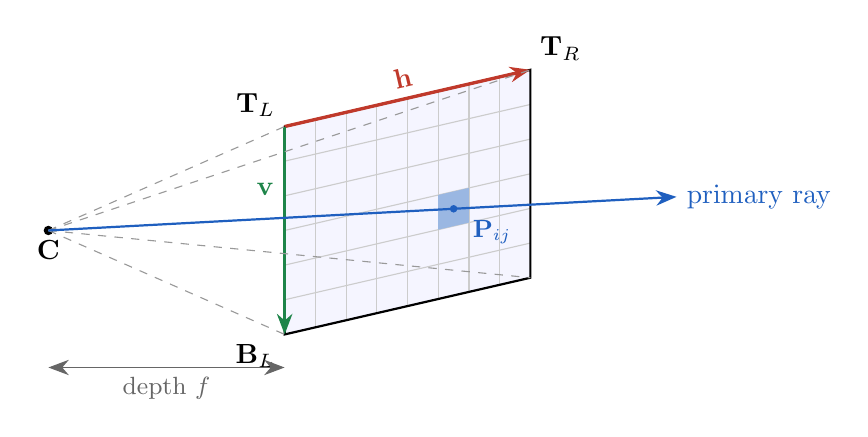
\begin{tikzpicture}[scale=1.2]
  \coordinate (TL) at (2.5,1.4);
  \coordinate (TR) at (5.1,2.0);
  \coordinate (BL) at (2.5,-0.8);
  \coordinate (BR) at (5.1,-0.2);
  \fill[blue!4] (TL) -- (TR) -- (BR) -- (BL) -- cycle;
  \foreach \k in {1,...,7}
     \draw[black!20] ($(TL)!\k/8!(TR)$) -- ($(BL)!\k/8!(BR)$);
  \foreach \k in {1,...,5}
     \draw[black!20] ($(TL)!\k/6!(BL)$) -- ($(TR)!\k/6!(BR)$);
  \draw[thick] (TL) -- (TR) -- (BR) -- (BL) -- cycle;
  % highlighted pixel
  \fill[cPrimary!45] ($(TL)+0.625*(2.6,0.6)+0.5*(0,-2.2)$) -- ++(0.325,0.075) -- ++(0,-0.3667) -- ++(-0.325,-0.075) -- cycle;
  \coordinate (P) at ($(TL)+0.6875*(2.6,0.6)+0.5833*(0,-2.2)$);
  \fill[cPrimary] (P) circle (0.04);
  % axes on plane
  \draw[->, very thick, cRefl] (TL) -- (TR) node[midway, above, sloped] {$\vv h$};
  \draw[->, very thick, cRefr] (TL) -- (BL) node[pos=0.3, left] {$\vv v$};
  \node[above left] at (TL) {$\vv T_L$};
  \node[above right] at (TR) {$\vv T_R$};
  \node[below left] at (BL) {$\vv B_L$};
  % eye
  \coordinate (E) at (0,0.3);
  \fill (E) circle (0.05) node[below] {$\vv C$};
  \draw[black!40, dashed] (E) -- (TL);
  \draw[black!40, dashed] (E) -- (TR);
  \draw[black!40, dashed] (E) -- (BL);
  \draw[black!40, dashed] (E) -- (BR);
  \draw[primary] (E) -- ($(E)!1.55!(P)$) node[right] {primary ray};
  \node[right, cPrimary] at ($(P)+(0.1,-0.25)$) {\small $\vv P_{ij}$};
  % depth
  \draw[<->, black!60] (0,-1.15) -- (2.5,-1.15) node[midway, below] {\small depth $f$};
\end{tikzpicture}
\caption{The image plane is a grid of pixels floating at distance $f$ in front of
the centre of projection. A pixel's point is found by walking $u$ of the way
along the top edge and $v$ of the way down the side.}
\label{fig:camera}
\end{figure}

\begin{inshort}
Compute the four plane corners in world space once. For every pixel, interpolate
its point on the plane and shoot a ray from the camera centre through it. Trace
that ray (with the full recursion budget) and write the returned colour into the
pixel.
\end{inshort}

\begin{algorithm}[h]
\caption{Generating primary rays}
\begin{algorithmic}[1]
\State $\vv T_L,\vv T_R,\vv B_L \gets$ plane corners mapped to world space
\State $\vv h\gets \vv T_R-\vv T_L,\quad \vv v\gets\vv B_L-\vv T_L$
\For{each row $i$, each column $j$}
   \State $u\gets j/(w-1),\quad v\gets i/(h-1)$
   \State $\vv P\gets \vv T_L + u\,\vv h + v\,\vv v$
   \State $\text{pixel}[i,j] \gets \textsc{Trace}\big(\text{ray from } \vv C \text{ towards } \vv P,\ D_{\max},\ n=1\big)$
\EndFor
\end{algorithmic}
\end{algorithm}

%===================================================================
\section{Finding the nearest hit}
%===================================================================

Given a ray, the tracer must find the \emph{closest} object it hits in front of
its origin. It does this by brute force: test every object, keep the hit with the
smallest positive $t$, and record the hit point $\vv X = \vv r(t)$, the surface
normal $\vv N$ there, and which object was hit. Exact intersection tests can be
expensive, so each object first goes through a cheap test.

\subsection{Cheap rejection with bounding boxes}

Every object stores an \emph{axis-aligned bounding box} (AABB), a box with faces
parallel to the coordinate planes that encloses it, enlarged by a tiny margin. A
box is the overlap of three \emph{slabs}, one per axis, where a slab is the
region between two parallel planes. A ray enters and leaves each slab at two
values of $t$:
\[
  t_1^{(k)} = \frac{\min_k - o_k}{d_k},\qquad t_2^{(k)} = \frac{\max_k - o_k}{d_k},
  \qquad k\in\{x,y,z\}.
\]
The ray is inside the box only while it is inside \emph{all three} slabs at
once, that is for $t\in[t_{\text{in}}, t_{\text{out}}]$ with
\[
  t_{\text{in}} = \max_k \min\big(t_1^{(k)},t_2^{(k)}\big),\qquad
  t_{\text{out}} = \min_k \max\big(t_1^{(k)},t_2^{(k)}\big).
\]
If $t_{\text{in}}>t_{\text{out}}$ (the intervals don't overlap) or
$t_{\text{out}}\le 0$ (the box is behind the ray), the object cannot be hit and
is skipped. If the ray is parallel to a slab, it either lies inside that slab or
misses the box outright. The test is \emph{conservative}: it may let through a
ray that then misses the object, but it never rejects a real hit.

\begin{figure}[h]
\centering
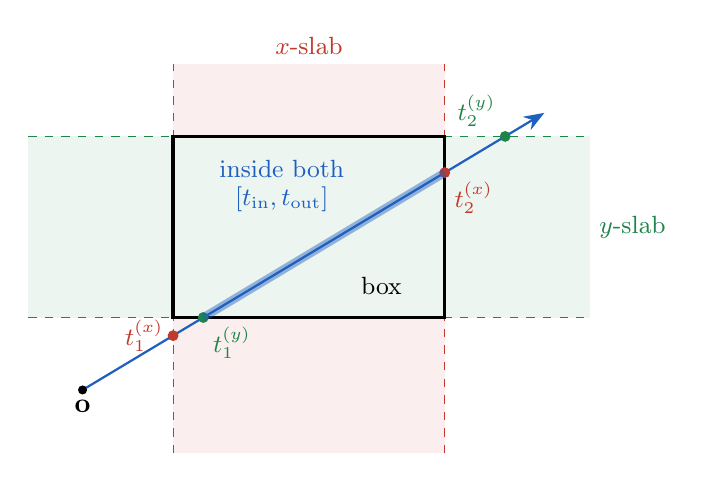
\begin{tikzpicture}[scale=1.15]
  % slabs
  \fill[cRefl!8] (1,-0.5) rectangle (4,3.8);
  \fill[cRefr!8] (-0.6,1) rectangle (5.6,3);
  \draw[cRefl, dashed] (1,-0.5) -- (1,3.8);
  \draw[cRefl, dashed] (4,-0.5) -- (4,3.8);
  \draw[cRefr, dashed] (-0.6,1) -- (5.6,1);
  \draw[cRefr, dashed] (-0.6,3) -- (5.6,3);
  \node[cRefl, above] at (2.5,3.8) {\small $x$-slab};
  \node[cRefr, right] at (5.6,2) {\small $y$-slab};
  \draw[very thick] (1,1) rectangle (4,3);
  \node at (3.3,1.35) {\small box};
  % ray: o=(0,0.2), d ~ (1,0.6)
  \draw[primary] (0,0.2) -- (5.1,3.26);
  \fill (0,0.2) circle (0.05) node[below] {$\vv o$};
  \foreach \p/\c/\l/\pos in {(1,0.8)/cRefl/{t_1^{(x)}}/left,
                             (4,2.6)/cRefl/{t_2^{(x)}}/below right,
                             (1.333,1.0)/cRefr/{t_1^{(y)}}/below right,
                             (4.667,3.0)/cRefr/{t_2^{(y)}}/above left}
     {\fill[\c] \p circle (0.06); \node[\c, \pos] at \p {\small $\l$};}
  \draw[line width=3pt, cPrimary, opacity=0.45] (1.333,1.0) -- (4,2.6);
  \node[cPrimary, align=center] at (2.2,2.45) {\small inside both\\[-2pt]\small$[t_{\text{in}},t_{\text{out}}]$};
\end{tikzpicture}
\caption{Slab test in 2D. The ray is inside the box exactly while it is inside
the $x$-slab \emph{and} the $y$-slab. The overlap (shaded on the ray) is
non-empty, so this ray is passed on to the exact intersection test.}
\end{figure}

\subsection{Exact intersection per shape}

\paragraph{Sphere.} A point is on a sphere (centre $\vv c$, radius $r$) when
$\lVert \vv x-\vv c\rVert^2=r^2$. Substituting the ray and writing
$\vv L = \vv o-\vv c$ gives a quadratic in $t$:
\[
  \underbrace{\dotp{\vv d}{\vv d}}_{a}t^2 + \underbrace{2\dotp{\vv d}{\vv L}}_{b}t
  + \underbrace{\dotp{\vv L}{\vv L}-r^2}_{c} = 0,\qquad
  t_{1,2} = \frac{-b\mp\sqrt{b^2-4ac}}{2a}.
\]
A negative discriminant means the ray misses. Otherwise the answer is the smaller
\emph{positive} root: $t_1$ if the ray starts outside the sphere, $t_2$ if it
starts inside (which happens for refracted rays travelling through glass). The
normal is $(\vv X-\vv c)/r$, which always points outward.

\begin{figure}[h]
\centering
\begin{subfigure}{0.48\textwidth}\centering
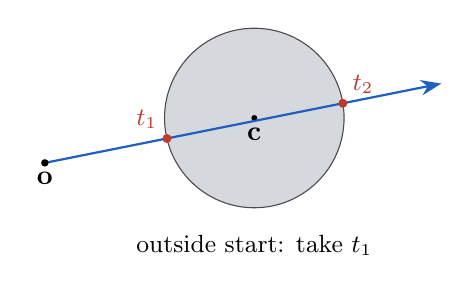
\begin{tikzpicture}[scale=0.95]
  \draw[solid] (2.5,0) circle (1.2);
  \fill (2.5,0) circle (0.04) node[below] {$\vv c$};
  \draw[primary] (-0.3,-0.6) -- (5,0.46);
  \fill (-0.3,-0.6) circle (0.05) node[below] {$\vv o$};
  \fill[cRefl] (1.332,-0.274) circle (0.06) node[above left] {\small $t_1$};
  \fill[cRefl] (3.684,0.197) circle (0.06) node[above right] {\small $t_2$};
  \node at (2.5,-1.7) {\small outside start: take $t_1$};
\end{tikzpicture}
\end{subfigure}
\begin{subfigure}{0.48\textwidth}\centering
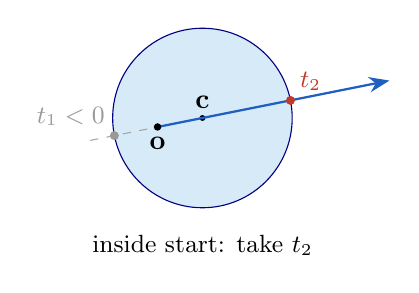
\begin{tikzpicture}[scale=0.95]
  \draw[glass] (2.5,0) circle (1.2);
  \fill (2.5,0) circle (0.04) node[above] {$\vv c$};
  \draw[black!35, dashed] (1.0,-0.3) -- (1.9,-0.12);
  \draw[primary] (1.9,-0.12) -- (5,0.5);
  \fill (1.9,-0.12) circle (0.05) node[below] {$\vv o$};
  \fill[black!40] (1.323,-0.235) circle (0.06) node[above left] {\small $t_1<0$};
  \fill[cRefl] (3.677,0.235) circle (0.06) node[above right] {\small $t_2$};
  \node at (2.5,-1.7) {\small inside start: take $t_2$};
\end{tikzpicture}
\end{subfigure}
\caption{Ray--sphere intersection. The two roots are the entry and exit
distances. A root behind the origin ($t\le 0$) is discarded.}
\end{figure}

\paragraph{Triangle (M\"oller--Trumbore).} Any point of the plane through
$\vv v_0,\vv v_1,\vv v_2$ can be written as $\vv v_0 + u\,\vv e_1 + v\,\vv e_2$
with edges $\vv e_1=\vv v_1-\vv v_0$, $\vv e_2=\vv v_2-\vv v_0$. Setting this
equal to $\vv o+t\vv d$ gives a $3\times3$ linear system in $(u,v,t)$, which is
solved with Cramer's rule using cross and dot products. The point lies inside the
triangle exactly when its \emph{barycentric coordinates} satisfy
\[
  u\ge 0,\qquad v\ge 0,\qquad u+v\le 1,
\]
and it counts as a hit only if $t>0$. If the system's determinant is close to
zero, the ray is parallel to the triangle. The normal is the same everywhere on
the triangle, $\vv e_1\times\vv e_2$ normalised, so it is computed once.

\paragraph{Quad.} A quad is split along a diagonal into two triangles. Both are
tested and the nearer hit wins.

\paragraph{Block (oriented box).} A block can be rotated, so the ray is first
moved into the block's own frame (subtract the centre, apply the inverse
rotation). There the block is an ordinary axis-aligned box centred at the
origin, and the same slab test as above gives the exact hit. This time it uses
$t_{\text{in}}$ if positive, otherwise $t_{\text{out}}$ (ray starting inside).
The normal is the face axis along which the local hit point is relatively
farthest out, i.e.\ the largest of $|x|/w,\ |y|/h,\ |z|/d$ with $w,h,d$ the
half-sizes. It is given the sign of that coordinate and rotated back to world
space.

\begin{figure}[h]
\centering
\begin{subfigure}{0.42\textwidth}\centering
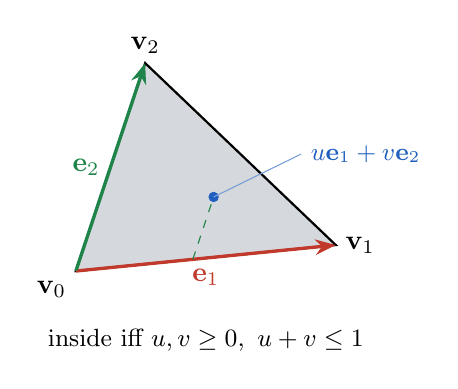
\begin{tikzpicture}[scale=1.1]
  \coordinate (A) at (0,0); \coordinate (B) at (3,0.3); \coordinate (Cc) at (0.8,2.4);
  \fill[cSolid] (A) -- (B) -- (Cc) -- cycle;
  \draw[thick] (A) -- (B) -- (Cc) -- cycle;
  \draw[->, very thick, cRefl] (A) -- (B) node[midway, below] {$\vv e_1$};
  \draw[->, very thick, cRefr] (A) -- (Cc) node[midway, left] {$\vv e_2$};
  \node[below left] at (A) {$\vv v_0$};
  \node[right] at (B) {$\vv v_1$};
  \node[above] at (Cc) {$\vv v_2$};
  \coordinate (P) at ($(A)+0.45*(3,0.3)+0.3*(0.8,2.4)$);
  \draw[cRefl, dashed] (A) -- ($(A)+0.45*(3,0.3)$);
  \draw[cRefr, dashed] ($(A)+0.45*(3,0.3)$) -- (P);
  \fill[cPrimary] (P) circle (0.06); \draw[cPrimary!60] (P) -- (2.6,1.35) node[right, cPrimary] {\small $u\vv e_1+v\vv e_2$};
  \node[align=center, font=\small] at (1.5,-0.8) {inside iff $u,v\ge0,\ u+v\le1$};
\end{tikzpicture}
\caption{Barycentric test.}
\end{subfigure}\hfill
\begin{subfigure}{0.55\textwidth}\centering
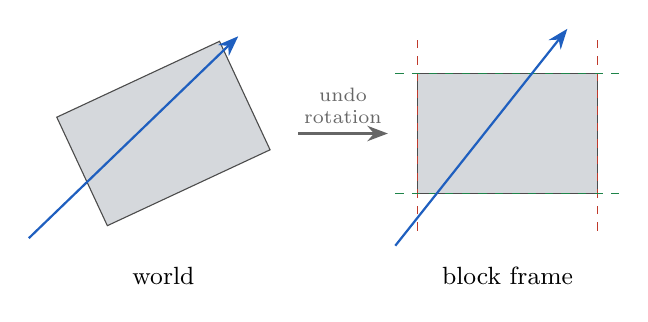
\begin{tikzpicture}[scale=0.95]
  \begin{scope}[rotate around={25:(1.2,1)}]
    \draw[solid] (0,0.2) rectangle (2.4,1.8);
  \end{scope}
  \draw[primary] (-0.6,-0.4) -- (2.2,2.3);
  \node at (1.2,-0.9) {\small world};
  \draw[->, thick, black!60] (3.0,1) -- (4.2,1) node[midway, above, font=\scriptsize, align=center] {undo\\rotation};
  \begin{scope}[xshift=4.6cm]
    \draw[solid] (0,0.2) rectangle (2.4,1.8);
    \draw[cRefl, dashed] (0,-0.3) -- (0,2.3);
    \draw[cRefl, dashed] (2.4,-0.3) -- (2.4,2.3);
    \draw[cRefr, dashed] (-0.3,0.2) -- (2.7,0.2);
    \draw[cRefr, dashed] (-0.3,1.8) -- (2.7,1.8);
    \draw[primary] (-0.3,-0.5) -- (2.0,2.4);
    \node at (1.2,-0.9) {\small block frame};
  \end{scope}
\end{tikzpicture}
\caption{A rotated block becomes an ordinary box.}
\end{subfigure}
\caption{Flat shapes use barycentric coordinates. Blocks are reduced to the
slab test.}
\end{figure}

\begin{inshort}
Loop over all objects. Skip an object if the ray misses its bounding box.
Otherwise run the exact test for its shape and keep the hit if it lies in front
of the origin and is nearer than the best hit so far. Afterwards, compute the
normal at the winning hit point.
\end{inshort}

\begin{algorithm}[h]
\caption{Nearest intersection}
\begin{algorithmic}[1]
\Function{NearestHit}{$\text{ray}$}
  \State $t^\star\gets\infty$, \ $\text{hit}\gets\text{none}$
  \ForEach{object $O$}
    \If{ray misses the bounding box of $O$} \textbf{continue} \EndIf
    \State $t \gets$ exact intersection of ray and $O$
    \If{$0 < t < t^\star$}
       \State $t^\star\gets t$, \ $\text{hit}\gets (O,\ \vv X=\vv r(t),\ \vv N = \text{normal of } O \text{ at } \vv X)$
    \EndIf
  \EndFor
  \State \Return hit
\EndFunction
\end{algorithmic}
\end{algorithm}

%===================================================================
\section{When a ray hits nothing: background and glow}
%===================================================================

\subsection{Background}

A ray that misses every object takes the background colour. That is either a
solid colour or a panoramic (equirectangular) image wrapped around the scene like
a sky dome. For the image:

\begin{enumerate}[leftmargin=1.6em]
  \item Pick a point far along the ray, $\vv S = \vv C + 15f\,\unit{\vv d}$. Using
        a far point rather than the bare direction gives a little
        \emph{parallax}: the background shifts slightly when the camera moves,
        and less so the farther away the point is chosen.
  \item Turn $\vv S$ into two angles, the \emph{yaw} (around the vertical axis)
        and the \emph{pitch} (above or below the horizon):
        \[
          \psi = \operatorname{atan2}(S_x, S_z)\in[-\pi,\pi],\qquad
          \theta = \operatorname{atan2}\big(S_y,\sqrt{S_x^2+S_z^2}\big)\in[-\tfrac\pi2,\tfrac\pi2].
        \]
  \item Rescale the angles to texture coordinates,
        $u = (\psi+\pi)/2\pi$ (wrapping around horizontally) and
        $v = (\theta+\pi/2)/\pi$, and read the nearest pixel.
\end{enumerate}

\begin{figure}[h]
\centering
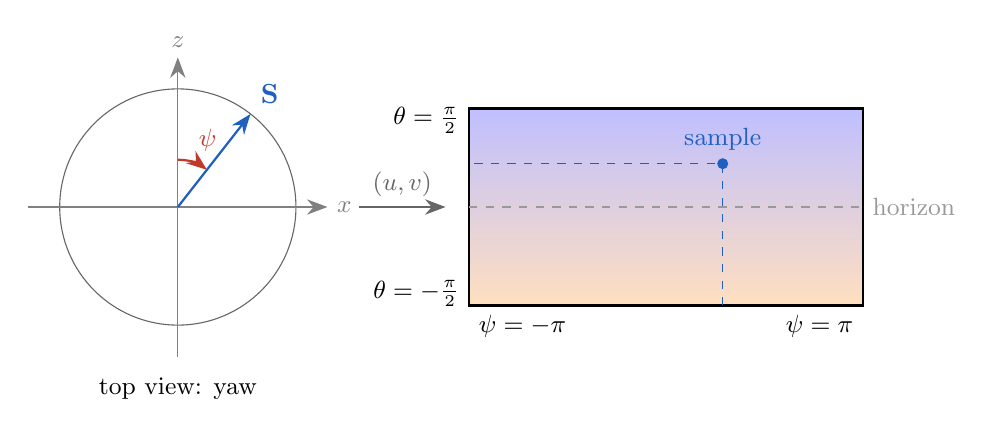
\begin{tikzpicture}[scale=1]
  % top view of direction sphere
  \draw[black!60] (0,0) circle (1.5);
  \draw[->, black!50] (0,-1.9) -- (0,1.9) node[above] {\small $z$};
  \draw[->, black!50] (-1.9,0) -- (1.9,0) node[right] {\small $x$};
  \draw[primary] (0,0) -- (52:1.5) node[above right] {$\vv S$};
  \draw[cRefl, thick, ->] (0,0.6) arc (90:52:0.6);
  \node[cRefl] at (0.38,0.85) {\small $\psi$};
  \node at (0,-2.3) {\small top view: yaw};
  % map arrow
  \draw[->, thick, black!60] (2.3,0) -- (3.4,0) node[midway, above] {\small $(u,v)$};
  % equirect image
  \begin{scope}[xshift=3.7cm, yshift=-1.25cm]
    \shade[top color=blue!25, bottom color=orange!25] (0,0) rectangle (5,2.5);
    \draw[thick] (0,0) rectangle (5,2.5);
    \draw[black!40, dashed] (0,1.25) -- (5,1.25) node[right] {\small horizon};
    \node[below right] at (0,0) {\small $\psi=-\pi$};
    \node[below left] at (5,0) {\small $\psi=\pi$};
    \node[left] at (0,0.15) {\small $\theta=-\tfrac\pi2$};
    \node[left] at (0,2.35) {\small $\theta=\tfrac\pi2$};
    \fill[cPrimary] (3.22,1.8) circle (0.07);
    \draw[cPrimary, dashed] (3.22,0) -- (3.22,1.8) -- (0,1.8);
    \node[cPrimary, above] at (3.22,1.85) {\small sample};
  \end{scope}
\end{tikzpicture}
\caption{Equirectangular lookup: the yaw angle picks the column and the pitch
angle picks the row, with the image wrapping horizontally like a cylinder.}
\end{figure}

\subsection{Glow halos around emissive spheres}

Spheres can be \emph{emissive}: they have an emission colour and strength. A
surface hit on such a sphere simply adds its emission to its colour. To make
lamps look like they glow, the tracer also adds a cheap \emph{halo}, an
approximation with no physical basis: every ray picks up some light when it
\emph{passes close} to an emitter.

For each emissive sphere (centre $\vv c$, radius $r$), find the point on the
travelled segment of the ray, $t\in[0,t_{\text{end}}]$, that is closest to the
centre. $t_{\text{end}}$ is the hit distance, or infinity for a ray that hits
nothing:
\[
  t^\ast = \operatorname{clamp}\big(\dotp{\vv c-\vv o}{\unit{\vv d}},\ 0,\ t_{\text{end}}\big),
  \qquad \delta = \lVert \vv r(t^\ast)-\vv c\rVert .
\]
If $\delta<r$, the ray actually hits the sphere and the surface takes care of it.
Otherwise the halo contribution decays exponentially with the gap
$\delta-r$ between the ray and the silhouette, in the spirit of the
Beer--Lambert attenuation law:
\[
  \text{glow} \mathrel{+}= 0.45\cdot s\cdot e^{-(\delta-r)/(0.3\,r)}\cdot \text{emission}.
\]
Here $s$ is the emission strength. The falloff scales with the radius, so large
lamps get wide halos. Glow is added both to rays that miss everything and to
rays that hit a surface after passing an emitter.

\begin{figure}[h]
\centering
\begin{subfigure}{0.5\textwidth}\centering
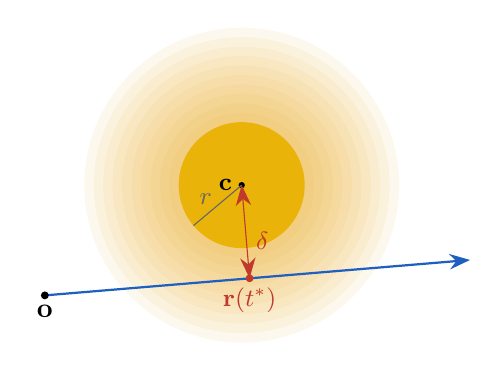
\begin{tikzpicture}[scale=1]
  \foreach \k in {10,...,1}
     \fill[cLight, opacity=0.07] (2.5,1.2) circle ({0.8+0.12*\k});
  \fill[cLight!80!yellow] (2.5,1.2) circle (0.8);
  \fill (2.5,1.2) circle (0.04) node[left] {\small $\vv c$};
  \draw[primary] (0,-0.2) -- (5.4,0.25);
  \fill (0,-0.2) circle (0.05) node[below] {$\vv o$};
  \coordinate (Q) at (2.6,0.017);
  \fill[cRefl] (Q) circle (0.05) node[below] {\small $\vv r(t^\ast)$};
  \draw[cRefl, <->] (Q) -- (2.5,1.2) node[pos=0.4, right] {\small $\delta$};
  \draw[black!60] (2.5,1.2) -- ++(-140:0.8) node[pos=0.55, above left, inner sep=1pt] {\small $r$};
\end{tikzpicture}
\end{subfigure}%
\begin{subfigure}{0.48\textwidth}\centering
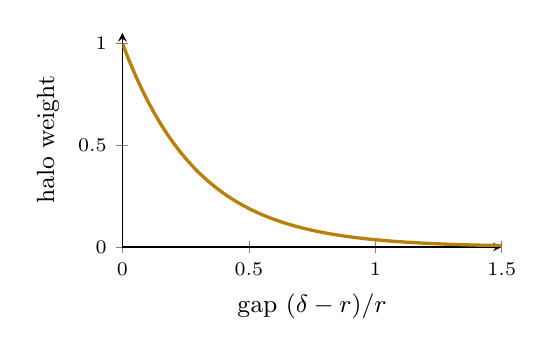
\begin{tikzpicture}
\begin{axis}[width=6.4cm, height=4.3cm, xlabel={gap $(\delta-r)/r$}, ylabel={halo weight},
  domain=0:1.5, samples=60, ymin=0, ymax=1.05, xmin=0, xmax=1.5, axis lines=left,
  every axis label/.style={font=\small}, tick label style={font=\scriptsize}]
  \addplot[cLight!80!black, very thick] {exp(-x/0.3)};
\end{axis}
\end{tikzpicture}
\end{subfigure}
\caption{Glow: the closer the ray passes to an emitter's silhouette, the more of
its emission it picks up. The weight halves roughly every $0.2r$.}
\end{figure}

\begin{inshort}
Miss $\Rightarrow$ background (solid colour or panorama lookup by yaw and pitch)
plus the glow of every emitter the ray passed near.
\end{inshort}

%===================================================================
\section{Direct lighting: the Phong model}
%===================================================================

When a ray hits a surface at $\vv X$ with unit normal $\vv N$, the first colour
computed is the \emph{direct} lighting: light that reaches $\vv X$ straight from
the light sources and bounces once toward the viewer. The tracer uses the
classic Phong model, with three kinds of light:

\begin{itemize}[leftmargin=1.4em]
  \item \textbf{ambient}: a constant amount, the same everywhere, that keeps
        shadows from going completely black;
  \item \textbf{point}: a light at a position $\vv Q$; the direction to it is
        $\vv L = (\vv Q-\vv X)/\lVert\vv Q-\vv X\rVert$;
  \item \textbf{directional}: a light infinitely far away (like the sun), given
        by one fixed direction $\vv L$.
\end{itemize}

Before rendering, all intensities $k_i$ are divided by their sum, so together
they add up to $1$ and a surface can never be over-lit just because the scene
has many lights.

\begin{figure}[h]
\centering
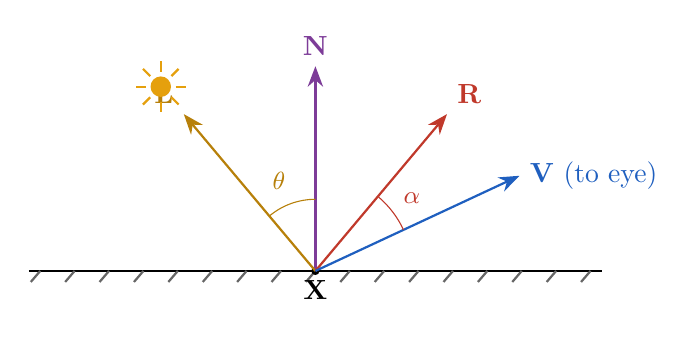
\begin{tikzpicture}[scale=1.3]
  \draw[thick, ground] (-2.8,0) -- (2.8,0);
  \fill (0,0) circle (0.04) node[below] {$\vv X$};
  \draw[normal] (0,0) -- (0,2) node[above] {$\vv N$};
  \draw[cLight!80!black, thick, ->] (0,0) -- (130:2) node[above left] {$\vv L$};
  \pic at (130:2.35) {lamp};
  \draw[reflray] (0,0) -- (50:2) node[above right] {$\vv R$};
  \draw[primary] (0,0) -- (25:2.2) node[right] {$\vv V$ (to eye)};
  \draw[cLight!80!black] (0,0.7) arc (90:130:0.7);
  \node[cLight!80!black] at (112:0.95) {\small $\theta$};
  \draw[cRefl] (50:0.95) arc (50:25:0.95);
  \node[cRefl] at (37:1.18) {\small $\alpha$};
\end{tikzpicture}
\caption{Phong vectors. Diffuse light depends on the angle $\theta$ between the
normal and the light. The specular highlight depends on the angle $\alpha$
between the mirrored light direction $\vv R$ and the direction $\vv V$ to the
viewer.}
\end{figure}

For every non-ambient light $i$, with shadow factor $b_i\in[0,1]$
(Section~\ref{sec:shadows}; $1$ means fully lit):
\begin{align*}
  I_{\text{diff}} &= \sum_{\text{ambient}} k_i \;+ \sum_{\text{point/dir}} k_i\,b_i\,\max\!\big(0,\dotp{\vv N}{\vv L_i}\big),\\
  I_{\text{spec}} &= \sum_{\text{point/dir}} k_i\,b_i\,\max\!\big(0,\dotp{\vv R_i}{\vv V}\big)^{s},
  \qquad \vv R_i = 2\dotp{\vv N}{\vv L_i}\vv N - \vv L_i,
\end{align*}
where $\vv V$ points from the surface to the camera and the exponent $s$ is the
material's shininess (small means a broad, dull highlight; large means a small,
sharp one). Both sums are capped at $1$. The \emph{albedo} $\vv a$ (the surface's
base colour) comes from the material or, for textured spheres and blocks, from
the texture at that point. The direct colour is then
\[
  \vv c_{\text{direct}} = \min\!\big(255,\ \vv a\,I_{\text{diff}} + 255\,I_{\text{spec}}\big).
\]
The diffuse term \emph{tints} the albedo, while the specular term adds
\emph{white}, which is why highlights look like reflections of the light rather
than brighter paint.

\begin{aside}{Where the albedo comes from (texture mapping)}
A textured sphere turns its normal into longitude and latitude and reads the
texture like a world map. A textured block works out which face was hit, uses
the two in-face coordinates as $(u,v)$, and repeats the pattern as many times as
requested. Either way, the result simply replaces the flat material colour
$\vv a$ above.
\end{aside}

\begin{inshort}
Start with the ambient light. For each other light, get its direction, ask the
shadow test how visible it is, then add a diffuse term ($\propto\cos\theta$) and
a specular term ($\propto\cos^s\alpha$), both scaled by that visibility.
Colour $=$ albedo $\times$ diffuse $+$ white $\times$ specular.
\end{inshort}

\begin{algorithm}[h]
\caption{Direct (Phong) shading at a hit point}
\begin{algorithmic}[1]
\Function{Direct}{$\vv X,\vv N,$ object}
  \State $I_d\gets 0,\ I_s\gets 0,\ \vv V\gets$ unit vector from $\vv X$ to camera
  \ForEach{light $i$}
    \If{ambient} $I_d\gets I_d+k_i$; \textbf{continue} \EndIf
    \State $b_i\gets\textsc{Shadow}(i,\vv X,\vv N)$
    \If{$b_i\approx 0$} \textbf{continue} \Comment{fully blocked} \EndIf
    \State $\vv L\gets$ direction to light $i$
    \State $I_s \gets I_s + k_i\,b_i \max(0,\dotp{\vv R}{\vv V})^s$ \Comment{only for shiny materials}
    \State $I_d \gets I_d + k_i\,b_i\max(0,\dotp{\vv N}{\vv L})$
  \EndFor
  \State \Return $\min\big(255,\ \text{albedo}(\vv X)\cdot\min(I_d,1) + 255\min(I_s,1)\big)$
\EndFunction
\end{algorithmic}
\end{algorithm}

%===================================================================
\section{Shadow rays}\label{sec:shadows}
%===================================================================

\subsection{The idea}

A point is in shadow with respect to a light if something sits between it and
that light. To find out, the tracer shoots a \textbf{shadow ray} from the hit
point $\vv X$ toward the light and checks whether any \emph{other} object is hit
before the ray gets there. An object never shadows itself. Since all the shapes
are convex, that is safe.

\begin{figure}[h]
\centering
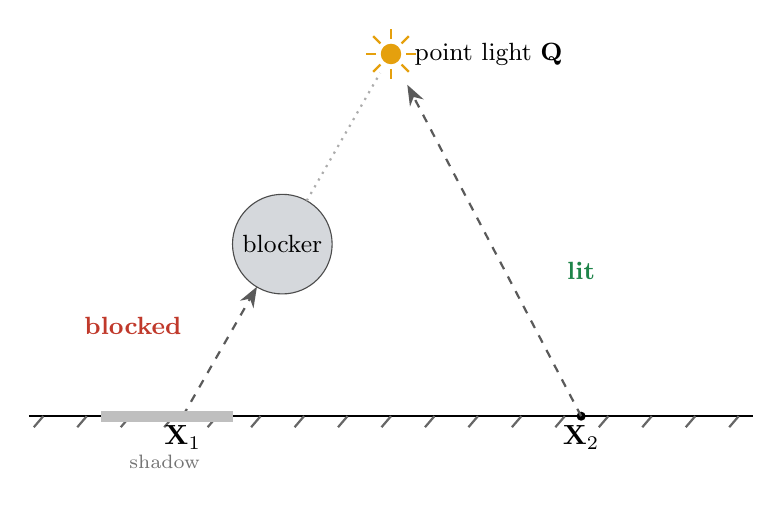
\begin{tikzpicture}[scale=1.15]
  \draw[thick, ground] (-0.5,0) -- (7.5,0);
  \pic at (3.5,4) {lamp};
  \node[right=5pt] at (3.5,4) {\small point light $\vv Q$};
  \draw[solid] (2.3,1.9) circle (0.55);
  \node at (2.3,1.9) {\small blocker};
  \fill (1.2,0) circle (0.05) node[below] {$\vv X_1$};
  \fill (5.6,0) circle (0.05) node[below] {$\vv X_2$};
  \draw[shadowray] (1.2,0) -- (2.02,1.43);
  \draw[cShadow!50, dotted, thick] (2.57,2.38) -- (3.38,3.79);
  \node[cRefl, font=\small] at (0.65,1.0) {\textbf{blocked}};
  \draw[shadowray] (5.6,0) -- (3.68,3.66);
  \node[cRefr, font=\small] at (5.6,1.6) {\textbf{lit}};
  \fill[black!25] (0.3,-0.06) rectangle (1.75,0.06);
  \node[black!55, font=\scriptsize] at (1.0,-0.5) {shadow};
\end{tikzpicture}
\caption{Shadow rays. From $\vv X_1$ the ray to the light hits the blocker at a
distance shorter than the light's, so $\vv X_1$ is in shadow. From $\vv X_2$ the
path is clear.}
\end{figure}

\subsection{Avoiding shadow acne}

The hit point $\vv X$ is computed in floating point, so it can land a hair
\emph{below} the surface. A shadow ray started there would immediately hit the
very surface it leaves and shadow itself, which shows up as dark speckles
(``shadow acne''). The fix is to push the shadow ray's origin a tiny distance
$\varepsilon$ off the surface, along the normal \emph{on the light's side}:
\[
  \vv o_{\text{shadow}} = \vv X + \varepsilon\,\operatorname{sign}\!\big(\dotp{\vv N}{\vv L}\big)\,\vv N .
\]
Choosing the side by the sign of $\dotp{\vv N}{\vv L}$ makes this work whether
the light is in front of the surface or behind it (for example a point inside a
glass object). The same trick is used for reflected and refracted rays, with a
larger offset.

\begin{figure}[h]
\centering
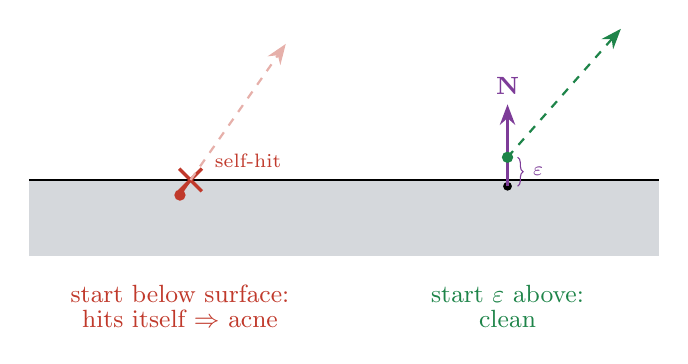
\begin{tikzpicture}[scale=1.6]
  \fill[cSolid] (-2.5,-0.6) rectangle (2.5,0);
  \draw[thick] (-2.5,0) -- (2.5,0);
  \begin{scope}[xshift=-1.3cm]
    \fill[cRefl] (0,-0.12) circle (0.045);
    \draw[cRefl, thick] (0,-0.12) -- (0.084,0);
    \draw[cRefl, very thick] (0.084,0) ++(-0.09,-0.09) -- ++(0.18,0.18) ++(0,-0.18) -- ++(-0.18,0.18);
    \draw[cRefl!40, thick, dashed, ->] (0.084,0) -- (0.84,1.08);
    \node[cRefl, font=\scriptsize, right] at (0.2,0.15) {self-hit};
    \node[cRefl, font=\small, align=center] at (0,-1.0) {start below surface:\\[-2pt]hits itself $\Rightarrow$ acne};
  \end{scope}
  \begin{scope}[xshift=1.3cm]
    \fill (0,-0.05) circle (0.035);
    \draw[normal] (0,-0.05) -- (0,0.6) node[above] {\small $\vv N$};
    \fill[cRefr] (0,0.18) circle (0.045);
    \draw[cNormal, decorate, decoration={brace, amplitude=2pt, mirror}] (0.08,-0.05) -- (0.08,0.18) node[midway, right=2pt, font=\scriptsize] {$\varepsilon$};
    \draw[shadowray, cRefr] (0,0.18) -- (0.9,1.2);
    \node[cRefr, font=\small, align=center] at (0,-1.0) {start $\varepsilon$ above:\\[-2pt]clean};
  \end{scope}
\end{tikzpicture}
\caption{Offsetting the origin along the normal prevents self-shadowing.}
\end{figure}

\subsection{How dark is the shadow? (soft-shadow heuristic)}

Real lights have a size, so shadows have soft edges. This tracer imitates that
softness with no extra rays at all. Instead of a hard ``lit / not lit'', the
shadow test returns a \emph{brightness} $b\in[0,1]$ ($1$: no shadow,
$0$: black).

\paragraph{Point lights.} Let $d$ be the distance from the (offset) origin to the
light and $t_{\text{occ}}$ the distance to the \emph{nearest} blocker on the
shadow ray. Only blockers with $0<t_{\text{occ}}<d$ count: something behind the
light cannot cast a shadow. If there is a blocker,
\[
  b = \dotp{\vv N}{\vv L}\cdot\frac{t_{\text{occ}}}{d}\quad(\text{clamped to }[0,1]).
\]
\begin{itemize}[leftmargin=1.4em]
  \item The ratio $t_{\text{occ}}/d$ makes a blocker \emph{close to the
        surface} cast a dark, solid shadow, while a blocker \emph{close to the
        light} casts a faint one. This matches what happens with a real light of
        some size: the further the blocker is from the surface, the more of the
        light can reach around it.
  \item The factor $\dotp{\vv N}{\vv L}$ darkens shadows further on surfaces
        that face away from the light.
\end{itemize}

\begin{figure}[h]
\centering
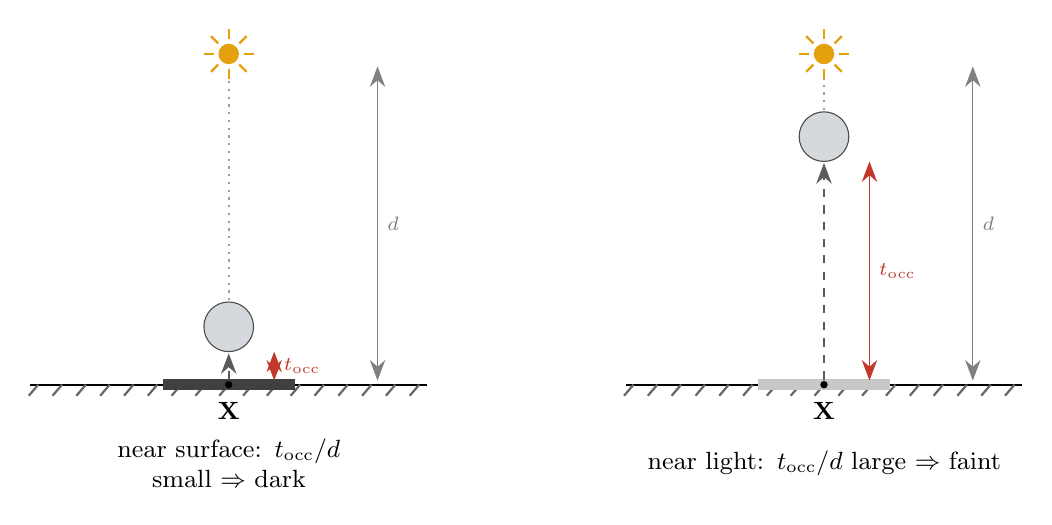
\begin{tikzpicture}[scale=1.05]
  \foreach \xs/\by/\lab/\shade in {0/0.7/{near surface: $t_{\text{occ}}/d$ small $\Rightarrow$ dark}/75,
                                   7.2/3.0/{near light: $t_{\text{occ}}/d$ large $\Rightarrow$ faint}/22} {
    \begin{scope}[xshift=\xs cm]
      \draw[thick, ground] (-0.6,0) -- (4.2,0);
      \pic at (1.8,4) {lamp};
      \fill[black!\shade] (1.0,-0.07) rectangle (2.6,0.07);
      \fill (1.8,0) circle (0.045) node[below=3pt] {\small $\vv X$};
      \draw[solid] (1.8,\by) circle (0.3);
      \draw[shadowray] (1.8,0.06) -- (1.8,{\by-0.32});
      \draw[cShadow!60, dotted, thick] (1.8,{\by+0.32}) -- (1.8,3.7);
      \draw[<->, cRefl] (2.35,0.05) -- (2.35,{\by-0.3}) node[midway, right, font=\scriptsize] {$t_{\text{occ}}$};
      \draw[<->, black!50] (3.6,0.05) -- (3.6,3.85) node[midway, right, font=\scriptsize] {$d$};
      \node[font=\small, align=center, text width=4.8cm] at (1.8,-0.95) {\lab};
    \end{scope}}
\end{tikzpicture}
\caption{Same light, same blocker size, different positions. Scaling the
brightness by $t_{\text{occ}}/d$ gives shadows that fade as the blocker moves
toward the light.}
\end{figure}

\paragraph{Directional lights.} A directional light is infinitely far away, so
there is no distance to compare against. Any blocker hit at $t>0$ counts, and
the brightness keeps only the orientation part, $b = \max(0,\dotp{\vv N}{\vv L})$.
One exception: if the surface faces away from the shadow ray \emph{and} so does
the blocker's surface where the shadow ray hits it, the point lies inside or
against that other object, and the blocker is ignored.

\paragraph{Ambient light} is never shadowed.

\begin{inshort}
For each point or directional light: offset the origin off the surface, toward
the light. Shoot a ray to the light and look for the nearest other object
between the surface and the light. No blocker means $b=1$. A blocker means a
partial brightness: \emph{orientation} $\times$ \emph{how far along the
blocker sits} (point lights), or just orientation (directional lights).
\end{inshort}

\begin{algorithm}[h]
\caption{Shadow factor for one light}
\begin{algorithmic}[1]
\Function{Shadow}{light, $\vv X,\vv N$}
  \State $\vv L\gets$ unit direction from $\vv X$ toward the light
  \State $\vv o\gets \vv X + \varepsilon\,\operatorname{sign}(\dotp{\vv N}{\vv L})\,\vv N$ \Comment{acne guard}
  \If{point light at $\vv Q$}
     \State $d\gets\lVert\vv Q-\vv o\rVert$; \ $t_{\text{occ}}\gets$ nearest hit in $(0,d)$ on ray $(\vv o,\vv L)$, ignoring self
     \If{no hit} \Return $1$ \EndIf
     \State \Return $\operatorname{clamp}\big(\dotp{\vv N}{\vv L}\cdot t_{\text{occ}}/d,\ 0,1\big)$
  \Else \Comment{directional}
     \If{no other object hit along $(\vv o,\vv L)$ (excluding ``inside'' cases)} \Return $1$ \EndIf
     \State \Return $\operatorname{clamp}(\dotp{\vv N}{\vv L},0,1)$
  \EndIf
\EndFunction
\end{algorithmic}
\end{algorithm}

%===================================================================
\section{Reflected rays}
%===================================================================

A mirror sends light back out at the same angle it came in, on the other side
of the normal. With a unit incoming direction $\vv I$ (pointing \emph{toward}
the surface) and a unit normal $\vv N$ on the incoming side, the reflected
direction is
\[
  \boxed{\ \vv R = \vv I - 2\dotp{\vv I}{\vv N}\,\vv N\ }
\]
The reason: $\dotp{\vv I}{\vv N}\vv N$ is the part of $\vv I$ that goes into
the surface. Subtracting it once leaves only the part along the surface.
Subtracting it a second time flips the into-surface part, so the ray now leaves
the surface (Figure~\ref{fig:reflect}).

\begin{figure}[h]
\centering
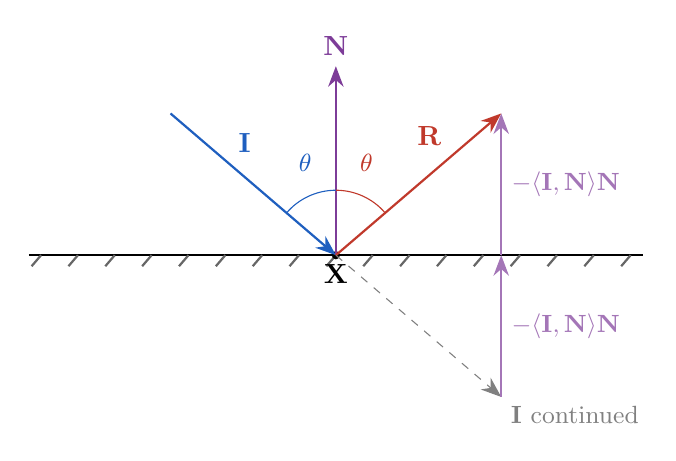
\begin{tikzpicture}[scale=1.5]
  \draw[thick, ground] (-2.6,0) -- (2.6,0);
  \fill (0,0) circle (0.035) node[below] {$\vv X$};
  \draw[normal] (0,0) -- (0,1.6) node[above] {$\vv N$};
  \draw[primary] (-1.4,1.2) -- (0,0) node[pos=0.35, above right] {$\vv I$};
  \draw[reflray] (0,0) -- (1.4,1.2) node[pos=0.7, above left] {$\vv R$};
  % construction
  \draw[black!50, dashed, ->] (0,0) -- (1.4,-1.2) node[below right, font=\small] {$\vv I$ continued};
  \draw[cNormal!70, ->, thick] (1.4,-1.2) -- (1.4,0) node[midway, right, font=\small] {$-\dotp{\vv I}{\vv N}\vv N$};
  \draw[cNormal!70, ->, thick] (1.4,0) -- (1.4,1.2) node[midway, right, font=\small] {$-\dotp{\vv I}{\vv N}\vv N$};
  \draw[cPrimary] (0,0.55) arc (90:139.4:0.55);
  \draw[cRefl] (0,0.55) arc (90:40.6:0.55);
  \node[cPrimary, font=\small] at (-0.26,0.78) {$\theta$};
  \node[cRefl, font=\small] at (0.26,0.78) {$\theta$};
\end{tikzpicture}
\caption{Reflection as ``take away the into-surface part twice''. The angle to the
normal is the same on both sides.}
\label{fig:reflect}
\end{figure}

The reflected ray starts at $\vv X$ pushed out by a small $\varepsilon$ along
the normal on the incoming side, which stops it from hitting the surface it is
leaving. It is traced recursively with one less unit of depth, and it travels
in the same medium as the incoming ray.

\paragraph{When is a reflected ray traced?} Whenever the surface is mirror-like
(reflectivity $\rho>0$) \emph{or} transparent ($\tau>0$). Transparent surfaces
reflect too, more so at grazing angles (Fresnel effect, next section), so they
need the reflected colour even if $\rho=0$.

\begin{inshort}
Mirror the incoming direction about the normal, start just above the surface,
and recursively trace. The returned colour is later blended in with weight
$\rho + \tau R_F$, where $R_F$ is the Fresnel reflectance of
Section~\ref{sec:refraction}.
\end{inshort}

\begin{algorithm}[h]
\caption{Reflected ray}
\begin{algorithmic}[1]
\State $\vv N\gets$ normal flipped to face the incoming ray
\State $\vv R\gets \vv I-2\dotp{\vv I}{\vv N}\vv N$
\State $\vv c_{\text{refl}}\gets\textsc{Trace}\big((\vv X+\varepsilon\vv N,\ \vv R),\ \text{depth}-1,\ n_1\big)$
\end{algorithmic}
\end{algorithm}

%===================================================================
\section{Refracted rays}\label{sec:refraction}
%===================================================================

\subsection{Snell's law}

Light slows down in glass or water. The \emph{index of refraction} $n$ says by
how much ($n=1$ for air, $\approx1.5$ for glass). When a ray crosses from a
medium with index $n_1$ into one with $n_2$, it bends according to Snell's law:
\[
  n_1\sin\theta_1 = n_2\sin\theta_2 .
\]
Going into a denser medium ($n_2>n_1$) bends the ray \emph{toward} the normal.
Going into a thinner one bends it \emph{away}.

\begin{figure}[h]
\centering
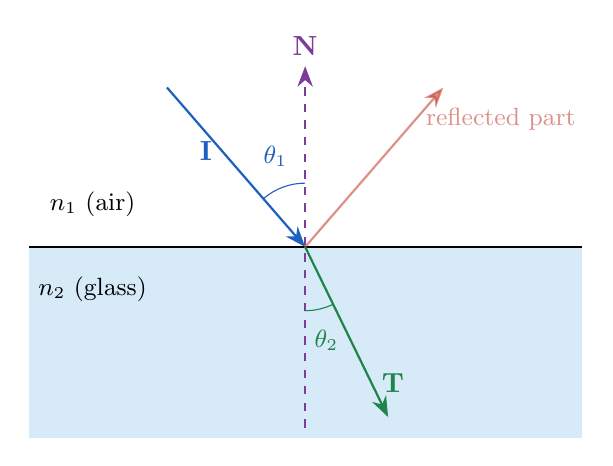
\begin{tikzpicture}[scale=1.35]
  \fill[cGlass] (-2.6,-1.8) rectangle (2.6,0);
  \draw[thick] (-2.6,0) -- (2.6,0);
  \node[font=\small] at (-2.0,0.4) {$n_1$ (air)};
  \node[font=\small] at (-2.0,-0.4) {$n_2$ (glass)};
  \draw[normal, dashed] (0,-1.7) -- (0,1.7) node[above] {$\vv N$};
  \draw[primary] (-1.3,1.5) -- (0,0) node[pos=0.4, left] {$\vv I$};
  \draw[refrray] (0,0) -- (0.78,-1.6) node[pos=0.8, right] {$\vv T$};
  \draw[reflray, opacity=0.55] (0,0) -- (1.3,1.5) node[pos=0.8, right] {\small reflected part};
  \draw[cPrimary] (0,0.6) arc (90:130.9:0.6);
  \node[cPrimary, font=\small] at (-0.28,0.85) {$\theta_1$};
  \draw[cRefr] (0,-0.6) arc (-90:-64:0.6);
  \node[cRefr, font=\small] at (0.2,-0.88) {$\theta_2$};
\end{tikzpicture}
\caption{Entering a denser medium: the transmitted ray $\vv T$ bends toward the
normal, so $\theta_2<\theta_1$. Some light is always reflected as well.}
\end{figure}

In vector form, with $\eta=n_1/n_2$, $\vv N$ facing the incoming side and
$\cos\theta_1 = -\dotp{\vv N}{\vv I}$:
\[
  k = 1-\eta^2\big(1-\cos^2\theta_1\big),\qquad
  \boxed{\ \vv T = \eta\,\vv I + \big(\eta\cos\theta_1-\sqrt{k}\big)\,\vv N\ }
\]
Here $k=\cos^2\theta_2$ follows from Snell's law. The first term keeps the
along-surface part of $\vv I$, scaled by $\eta$. The second term sets the
into-surface part so that the result has unit length.

\subsection{Total internal reflection}

If $k<0$, there is no real $\theta_2$: the ray is trying to leave a dense medium
at too shallow an angle (past the \emph{critical angle}
$\theta_c=\arcsin(n_2/n_1)$). Then no light gets through and the surface acts as
a perfect mirror. This is \textbf{total internal reflection} (TIR), the reason
diamonds sparkle and the edges of a glass ball look silvery. In this case the
tracer traces no refracted ray and gives all of the transmitted share to the
reflected ray.

\begin{figure}[h]
\centering
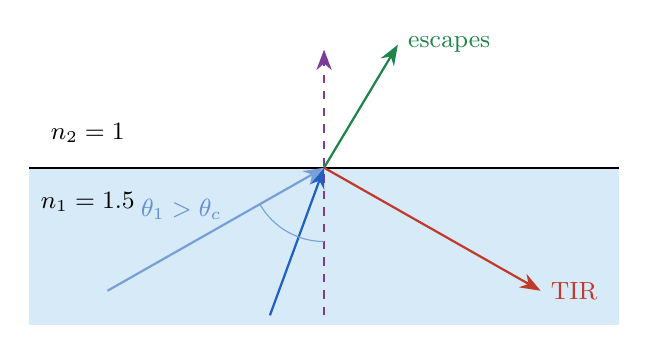
\begin{tikzpicture}[scale=1.25]
  \fill[cGlass] (-3,-1.6) rectangle (3,0);
  \draw[thick] (-3,0) -- (3,0);
  \node[font=\small] at (-2.4,0.35) {$n_2=1$};
  \node[font=\small] at (-2.4,-0.35) {$n_1=1.5$};
  \draw[normal, dashed] (0,-1.5) -- (0,1.2);
  % below critical: refracts out
  \draw[primary] (-0.55,-1.5) -- (0,0);
  \draw[refrray] (0,0) -- (0.75,1.25) node[right, font=\small] {escapes};
  % at/above critical: TIR
  \draw[primary, cPrimary!60] (-2.2,-1.25) -- (0,0);
  \draw[reflray] (0,0) -- (2.2,-1.25) node[right, font=\small] {TIR};
  \draw[cPrimary!60] (0,-0.75) arc (-90:-150.4:0.75);
  \node[font=\small, cPrimary!70] at (-1.45,-0.42) {$\theta_1>\theta_c$};
\end{tikzpicture}
\caption{Leaving glass: steep rays escape (bent away from the normal), but past
the critical angle ($\approx 41.8^\circ$ for glass) all light reflects back
inside.}
\end{figure}

\subsection{Entering or leaving? Orienting the normal and finding $n_1,n_2$}

Object normals always point \emph{outward}. The sign of $\dotp{\vv N}{\vv I}$
tells the tracer which side the ray comes from:

\begin{itemize}[leftmargin=1.4em]
  \item $\dotp{\vv N}{\vv I}<0$: the ray is \textbf{entering} the object. Use
        $\vv N$ as it is. $n_1$ is the medium the ray is travelling in and $n_2$
        the object's index.
  \item $\dotp{\vv N}{\vv I}>0$: the ray is \textbf{leaving} the object. Flip
        the normal ($-\vv N$) so it faces the incoming side. $n_1$ is the
        object's index and $n_2$ that of whatever surrounds the object.
\end{itemize}

Every ray carries the index of the medium it is in, which starts at $1$ (air)
for primary rays. A refracted child ray carries $n_2$; a reflected child ray
carries $n_1$. This is how the tracer knows it is inside glass.

\paragraph{What surrounds the object?} Objects can be nested, for example an air
bubble inside a glass block. To find the medium on the outside of a surface, the
tracer places a \emph{probe} point a little outside the surface, along the
outward normal, and asks each other closed solid (spheres and blocks) whether
the probe is inside it. If one contains it, its index is the surrounding index;
otherwise it is air ($n=1$). A cheap bounding-box check comes first here too.

\begin{figure}[h]
\centering
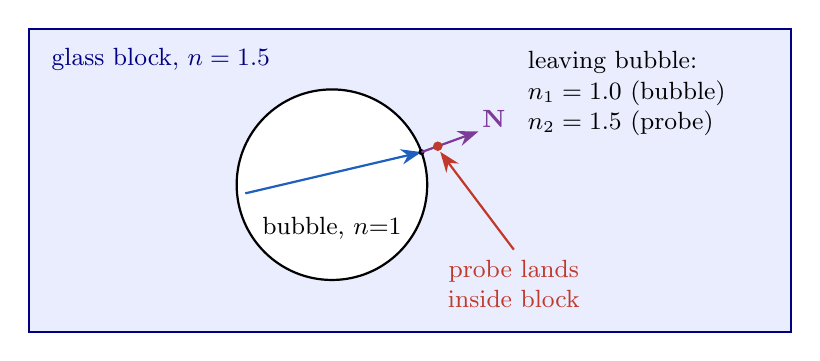
\begin{tikzpicture}[scale=1.1]
  \fill[cGlass!70!blue!20] (-0.5,-1.7) rectangle (8.3,1.8);
  \draw[thick, blue!50!black] (-0.5,-1.7) rectangle (8.3,1.8);
  \node[font=\small, blue!50!black, anchor=west] at (-0.35,1.45) {glass block, $n=1.5$};
  \draw[thick, fill=white] (3,0) circle (1.1);
  \node[font=\small] at (3,-0.5) {bubble, $n{=}1$};
  % ray travelling inside the bubble, about to leave it
  \draw[primary] (2.0,-0.1) -- (4.034,0.376);
  \fill (4.034,0.376) circle (0.035);
  \draw[normal] (4.034,0.376) -- (4.692,0.615) node[above right, font=\small, inner sep=1pt] {$\vv N$};
  \fill[cRefl] (4.222,0.444) circle (0.055);
  \draw[cRefl, <-, thick] (4.25,0.38) -- (5.1,-0.75) node[below, font=\small, align=center] {probe lands\\inside block};
  \node[align=left, font=\small, anchor=north west] at (5.15,1.65) {leaving bubble:\\$n_1=1.0$ (bubble)\\$n_2=1.5$ (probe)};
\end{tikzpicture}
\caption{Nested media. A ray travelling inside an air bubble reaches the
bubble's surface. The probe just outside that surface lands inside the glass
block, so the ray continues into $n_2=1.5$, not into air.}
\end{figure}

\subsection{How much is reflected? Fresnel and Schlick}

A transparent surface does not let all its light through. The fraction it
reflects, $R_F$, rises sharply toward grazing angles. That is why a lake mirrors
the far shore but is see-through at your feet. The exact Fresnel equations are
expensive, so the tracer uses \textbf{Schlick's approximation}:
\[
  R_0 = \left(\frac{n_1-n_2}{n_1+n_2}\right)^2,\qquad
  R_F(\theta_1) = R_0 + (1-R_0)\,(1-\cos\theta_1)^5 .
\]
$R_0$ is the reflectance when looking straight on (about $4\%$ for air/glass).

\begin{figure}[h]
\centering
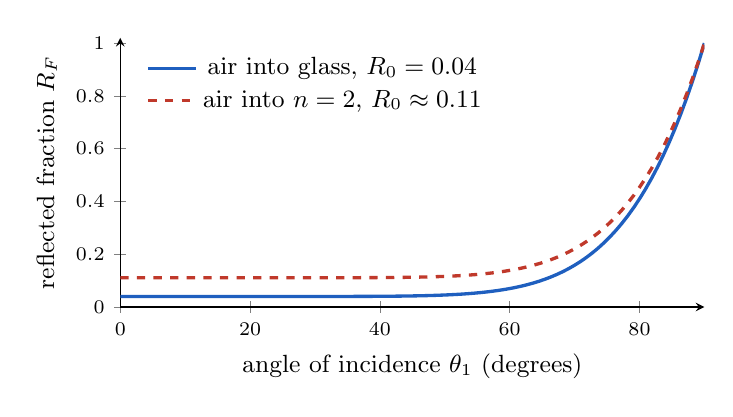
\begin{tikzpicture}
\begin{axis}[width=9cm, height=5cm, xlabel={angle of incidence $\theta_1$ (degrees)},
  ylabel={reflected fraction $R_F$}, domain=0:90, samples=100, xmin=0, xmax=90,
  ymin=0, ymax=1.02, axis lines=left, legend pos=north west, legend style={font=\small, draw=none},
  every axis label/.style={font=\small}, tick label style={font=\scriptsize}]
  \addplot[cPrimary, very thick] {0.04 + 0.96*(1-cos(x))^5};
  \addlegendentry{air into glass, $R_0=0.04$}
  \addplot[cRefl, very thick, dashed] {0.111 + 0.889*(1-cos(x))^5};
  \addlegendentry{air into $n=2$, $R_0\approx0.11$}
\end{axis}
\end{tikzpicture}
\caption{Schlick's curve: almost flat until about $60^\circ$, then climbing fast
to full reflection at grazing incidence.}
\end{figure}

\subsection{Tint}

Coloured glass shades the light that passes through it. A tint strength
$\kappa\in[0,1]$, scaled by the transparency $\tau$, blends each colour channel
of the refracted colour toward the object's own colour $\vv a$:
\[
  c_{\text{refr}} \leftarrow c_{\text{refr}}\cdot\Big[(1-\tau\kappa) + \tau\kappa\,\frac{a}{255}\Big]
  \quad\text{(per channel)}.
\]
With $\kappa=0$ the glass is perfectly clear. With $\kappa=1$ and full
transparency, each channel of what is seen through it is multiplied by the
glass's colour.

\begin{inshort}
Find out whether the ray is entering or leaving. Orient the normal and pick
$(n_1,n_2)$, probing for the surrounding medium if needed. Compute Schlick's
$R_F$. Bend the ray with vector Snell. If $k<0$ it is TIR, so no refracted ray
and the reflected one takes over. Otherwise start just past the surface along
$\vv T$, trace recursively in medium $n_2$ and tint the result.
\end{inshort}

\begin{algorithm}[h]
\caption{Refracted ray}
\begin{algorithmic}[1]
\If{$\dotp{\vv N}{\vv I}<0$} \Comment{entering}
  \State $\vv N'\gets\vv N$, \ $n_1\gets n_{\text{ray}}$, \ $n_2\gets n_{\text{object}}$
\Else \Comment{leaving}
  \State $\vv N'\gets-\vv N$, \ $n_1\gets n_{\text{object}}$, \ $n_2\gets \textsc{SurroundingIndex}(\vv X)$
\EndIf
\State $\eta\gets n_1/n_2$, \ $\cos\theta_1\gets-\dotp{\vv N'}{\vv I}$, \ $R_F\gets$ Schlick$(n_1,n_2,\cos\theta_1)$
\State $k\gets1-\eta^2(1-\cos^2\theta_1)$
\If{$k<0$} \State TIR: no refracted ray, move its weight to reflection
\Else
  \State $\vv T\gets \eta\vv I+(\eta\cos\theta_1-\sqrt k)\vv N'$
  \State $\vv c_{\text{refr}}\gets\textsc{Trace}\big((\vv X+\varepsilon\vv T,\ \vv T),\ \text{depth}-1,\ n_2\big)$
  \State apply tint toward the object colour
\EndIf
\end{algorithmic}
\end{algorithm}

%===================================================================
\section{Blending everything at a hit point}
%===================================================================

A surface can be part matte, part mirror and part glass at once. Its material
gives a reflectivity $\rho\in[0,1]$ and a transparency $\tau\in[0,1]$. Together
with the Fresnel reflectance $R_F$, these decide how much each colour
contributes:
\begin{align*}
  w_t &= \tau\,(1-R_F) && \text{transmitted (refracted) share}\\
  w_r &= \rho + \tau\,R_F && \text{reflected share: mirror part + glass reflection}\\
  w_d &= 1-\min(w_r+w_t,\ 1) && \text{whatever remains goes to direct lighting}
\end{align*}
Under total internal reflection, $w_t=0$ and $w_r\leftarrow\min(1,w_r+\tau)$.
The direct colour of a transparent surface is also dimmed by $(1-\tau)$ before
blending, because a clear object has little ``paint'' of its own. The final
colour is
\[
  \boxed{\ \vv c = w_d\,(1-\tau)\,\vv c_{\text{direct}} + w_r\,\vv c_{\text{refl}} + w_t\,\vv c_{\text{refr}} + \text{glow}\ }
\]

\begin{figure}[h]
\centering
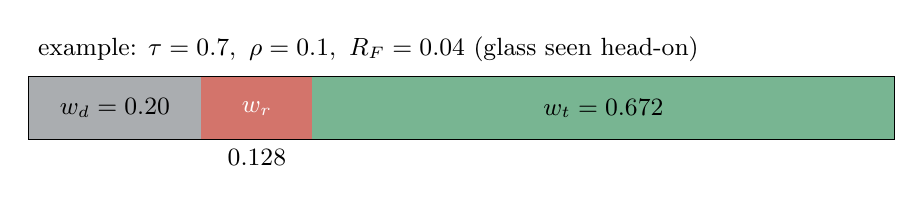
\begin{tikzpicture}[scale=1]
  % example: tau=0.7, rho=0.1, R=0.04 -> w_t=0.672, w_r=0.128, w_d=0.2
  \def\L{11}
  \fill[cSolid!80!black] (0,0) rectangle ({0.2*\L},0.8);
  \fill[cRefl!70] ({0.2*\L},0) rectangle ({0.328*\L},0.8);
  \fill[cRefr!60] ({0.328*\L},0) rectangle (\L,0.8);
  \draw (0,0) rectangle (\L,0.8);
  \node[font=\small] at ({0.1*\L},0.4) {$w_d=0.20$};
  \node[font=\small, text=white] at ({0.264*\L},0.4) {$w_r$};
  \node[font=\small] at ({0.664*\L},0.4) {$w_t=0.672$};
  \node[font=\small, below] at ({0.264*\L},0) {$0.128$};
  \node[font=\small, anchor=west] at (0,1.15) {example: $\tau=0.7,\ \rho=0.1,\ R_F=0.04$ (glass seen head-on)};
\end{tikzpicture}
\caption{How one pixel's colour is split between a mostly transparent, slightly
mirrored surface's three sources.}
\end{figure}

\paragraph{When does the recursion stop?} At a hit, no child rays are spawned
(the colour is just the direct light plus any emission) if
\begin{itemize}[leftmargin=1.4em]
  \item the depth budget is used up, or
  \item the surface is neither reflective nor transparent ($\rho\approx0$ and
        $\tau\approx0$).
\end{itemize}
Otherwise, every hit spawns a reflected ray and, if transparent, a refracted ray
as well. The rays therefore form a binary \emph{ray tree}, with shadow rays as
leaves hanging off every node (Figure~\ref{fig:tree}). The tree has at most
$2^{D}$ leaves, which is why the depth budget $D$ is the main control over speed.

\begin{figure}[h]
\centering
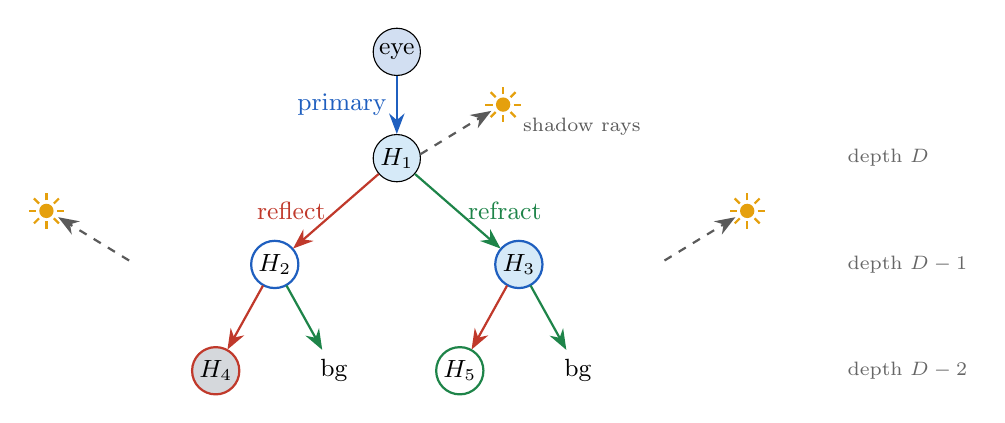
\begin{tikzpicture}[
  level distance=1.35cm,
  level 1/.style={sibling distance=6.2cm},
  level 2/.style={sibling distance=3.1cm},
  level 3/.style={sibling distance=1.5cm},
  every node/.style={font=\small},
  hit/.style={circle, draw, fill=white, minimum size=6mm, inner sep=0pt},
  edge from parent/.style={draw, thick, ->}]
  \node[hit, fill=cPrimary!20] {eye}
    child {node[hit, fill=cGlass] {$H_1$}
      child {node[hit] {$H_2$}
        child {node[hit, fill=cSolid] {$H_4$} edge from parent[cRefl]}
        child {node {bg} edge from parent[cRefr]}
        edge from parent[cRefl] node[left, cRefl] {reflect}}
      child {node[hit, fill=cGlass] {$H_3$}
        child {node[hit] {$H_5$} edge from parent[cRefl]}
        child {node {bg} edge from parent[cRefr]}
        edge from parent[cRefr] node[right, cRefr] {refract}}
      edge from parent[cPrimary] node[left, cPrimary] {primary}};
  % shadow leaves
  \foreach \x/\y/\s in {0/-1.35/1, -3.1/-2.7/-1, 3.1/-2.7/1} {
    \draw[shadowray] (\x+\s*0.3,\y+0.05) -- ++(\s*0.9,0.55);
    \pic[scale=0.7] at (\x+\s*1.35,\y+0.68) {lamp};
  }
  \node[cShadow, font=\scriptsize] at (2.35,-0.95) {shadow rays};
  \node[font=\scriptsize, black!60, right] at (5.6,-1.35) {depth $D$};
  \node[font=\scriptsize, black!60, right] at (5.6,-2.7) {depth $D-1$};
  \node[font=\scriptsize, black!60, right] at (5.6,-4.05) {depth $D-2$};
\end{tikzpicture}
\caption{The ray tree for one pixel. Each reflective/transparent hit branches
into a reflected (red) and a refracted (green) child. Every hit also sends shadow
rays to the lights for its direct term. ``bg'' marks rays that escape to the
background. Colours flow \emph{up} the tree and are blended at each node.}
\label{fig:tree}
\end{figure}

%===================================================================
\section{Post-processing: gamma correction}
%===================================================================

Once every pixel has a colour, the image is gamma-corrected. Each 8-bit value is
remapped through
\[
  c' = 255\left(\frac{c}{255}\right)^{\gamma}.
\]
The map is precomputed into a 256-entry lookup table, so applying it is just one
array read per channel. $\gamma<1$ lifts the dark tones (useful because the
weights above tend to darken the image), while $\gamma>1$ deepens them.

\begin{figure}[h]
\centering
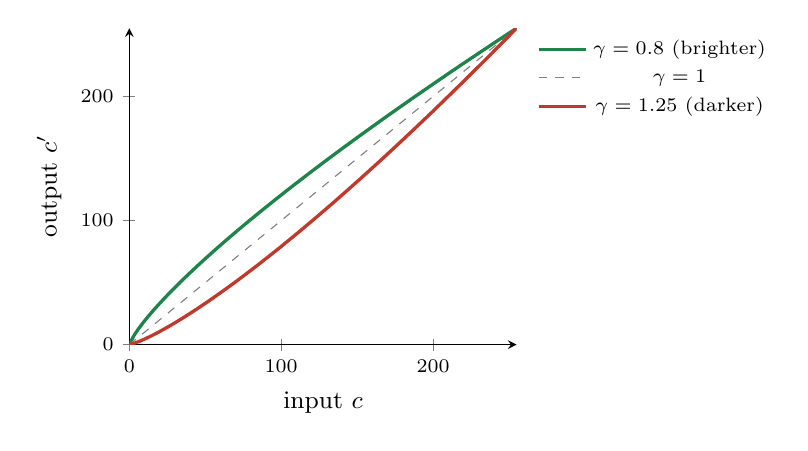
\begin{tikzpicture}
\begin{axis}[width=6.5cm, height=5.6cm, xlabel={input $c$}, ylabel={output $c'$},
  domain=0:255, samples=80, xmin=0, xmax=255, ymin=0, ymax=255, axis lines=left,
  legend pos=outer north east, legend style={font=\scriptsize, draw=none},
  every axis label/.style={font=\small}, tick label style={font=\scriptsize}]
  \addplot[cRefr, very thick] {255*(x/255)^0.8}; \addlegendentry{$\gamma=0.8$ (brighter)}
  \addplot[black!50, dashed] {x};              \addlegendentry{$\gamma=1$}
  \addplot[cRefl, very thick] {255*(x/255)^1.25}; \addlegendentry{$\gamma=1.25$ (darker)}
\end{axis}
\end{tikzpicture}
\caption{Gamma curves.}
\end{figure}

%===================================================================
\section{Putting it all together}
%===================================================================

The pieces now fit into one recursive procedure. \textsc{Render} runs once.
\textsc{Trace} is called for every primary ray and then calls itself for
reflected and refracted rays. \textsc{Direct} and \textsc{Shadow} handle the
lighting at each hit.

\begin{algorithm}[p]
\caption{The complete freestyle ray tracer: rendering and tracing}
\label{alg:full}
\begin{algorithmic}[1]
\Function{Render}{scene, camera, $D_{\max}$, $\gamma$}
  \State divide every light intensity by the sum of all intensities
  \State collect the emissive spheres (for glow)
  \State $\vv T_L,\vv T_R,\vv B_L\gets$ image-plane corners in world space; \ $\vv h\gets\vv T_R-\vv T_L$, \ $\vv v\gets\vv B_L-\vv T_L$
  \For{each pixel $(i,j)$}
     \State $\vv P\gets \vv T_L + \tfrac{j}{w-1}\vv h + \tfrac{i}{h-1}\vv v$
     \State $\text{image}[i,j]\gets\textsc{Trace}\big(\text{ray}(\vv C\to\vv P),\ D_{\max},\ 1\big)$
  \EndFor
  \State apply gamma $c\mapsto 255(c/255)^\gamma$ to every channel
\EndFunction
\Statex
\Function{Trace}{ray $(\vv o,\vv I)$, depth, $n_{\text{ray}}$}
  \State $(O,\ \vv X,\ \vv N,\ t_{\text{hit}})\gets\textsc{NearestHit}(\text{ray})$ \Comment{AABB cull + exact tests}
  \If{no hit}
     \State \Return $\textsc{Background}(\vv I) + \textsc{Glow}(\text{ray}, \infty)$
  \EndIf
  \State $\rho,\tau\gets$ reflectivity and transparency of $O$
  \State $\vv c_d\gets(1-\tau)\cdot\textsc{Direct}(\vv X,\vv N,O)$ \Comment{Phong + shadow rays}
  \If{$\text{depth}=0$ \textbf{or} ($\rho\approx0$ \textbf{and} $\tau\approx0$)}
     \State \Return $\vv c_d + \text{emission}(O)$ \Comment{leaf of the ray tree}
  \EndIf
  \Statex \hspace{\algorithmicindent}\textit{--- orientation ---}
  \If{$\dotp{\vv N}{\vv I}<0$} $\vv N'\gets\vv N$; \ $n_1\gets n_{\text{ray}}$; \ $n_2\gets n_O$ \Comment{entering}
  \Else\ \ $\vv N'\gets-\vv N$; \ $n_1\gets n_O$; \ $n_2\gets\textsc{SurroundingIndex}(\vv X)$ \Comment{leaving}
  \EndIf
  \State $\eta\gets n_1/n_2$, \ $\cos\theta_1\gets-\dotp{\vv N'}{\vv I}$
  \Statex \hspace{\algorithmicindent}\textit{--- reflection ---}
  \State $\vv R\gets\vv I-2\dotp{\vv I}{\vv N'}\vv N'$
  \State $\vv c_r\gets\textsc{Trace}\big((\vv X+\varepsilon\vv N',\ \vv R),\ \text{depth}-1,\ n_1\big)$
  \Statex \hspace{\algorithmicindent}\textit{--- refraction ---}
  \State $R_F\gets R_0+(1-R_0)(1-\cos\theta_1)^5$, \quad $R_0=\big(\frac{n_1-n_2}{n_1+n_2}\big)^2$
  \State $w_t\gets\tau(1-R_F)$, \ $w_r\gets\rho+\tau R_F$, \ $\vv c_t\gets\vv 0$
  \If{$\tau>0$}
     \State $k\gets1-\eta^2(1-\cos^2\theta_1)$
     \If{$k<0$} \Comment{total internal reflection}
        \State $w_t\gets0$, \ $w_r\gets\min(1,\ w_r+\tau)$
     \Else
        \State $\vv T\gets\eta\vv I+(\eta\cos\theta_1-\sqrt k)\vv N'$
        \State $\vv c_t\gets\textsc{Trace}\big((\vv X+\varepsilon\vv T,\ \vv T),\ \text{depth}-1,\ n_2\big)$
        \State $\vv c_t\gets \vv c_t\odot\big[(1-\tau\kappa)+\tau\kappa\,\vv a_O/255\big]$ \Comment{tint}
     \EndIf
  \EndIf
  \Statex \hspace{\algorithmicindent}\textit{--- blend ---}
  \State $w_d\gets1-\min(w_r+w_t,1)$
  \State \Return $w_d\,\vv c_d + w_r\,\vv c_r + w_t\,\vv c_t + \textsc{Glow}(\text{ray}, t_{\text{hit}})$
\EndFunction
\end{algorithmic}
\end{algorithm}

\begin{algorithm}[t]
\caption{The complete ray tracer, continued: lighting at a hit}
\label{alg:full2}
\begin{algorithmic}[1]
\Function{Direct}{$\vv X,\vv N,O$}
  \State $I_d\gets\sum_{\text{ambient}}k_i$, \ $I_s\gets0$, \ $\vv V\gets$ unit vector from $\vv X$ to camera
  \ForEach{point or directional light $i$}
     \State $b\gets\textsc{Shadow}(i,\vv X,\vv N)$; \ \textbf{if} $b\approx0$ \textbf{continue}
     \State $I_d\gets I_d+k_i\,b\max(0,\dotp{\vv N}{\vv L_i})$; \ $I_s\gets I_s+k_i\,b\max(0,\dotp{\vv R_i}{\vv V})^{s}$
  \EndFor
  \State \Return $\min\big(255,\ \text{albedo}_O(\vv X)\min(I_d,1)+255\min(I_s,1)\big)$
\EndFunction
\Statex
\Function{Shadow}{light $i$, $\vv X,\vv N$}
  \State $\vv o\gets\vv X+\varepsilon\operatorname{sign}(\dotp{\vv N}{\vv L_i})\vv N$
  \State find nearest other object on ray $(\vv o,\vv L_i)$, before the light if it is a point light
  \If{none} \Return 1 \EndIf
  \If{point light} \Return $\operatorname{clamp}\big(\dotp{\vv N}{\vv L_i}\cdot t_{\text{occ}}/d,\ 0,1\big)$
  \Else\ \Return $\operatorname{clamp}(\dotp{\vv N}{\vv L_i},0,1)$
  \EndIf
\EndFunction
\end{algorithmic}
\end{algorithm}

\paragraph{Reading the algorithm as a story.} For each pixel, a ray leaves the
eye. It either escapes to the sky (background plus any glow it passed through)
or lands on a surface. There it gathers light from the lamps, with each lamp
dimmed by its shadow ray. If the surface is plain, that is the answer. If it is
shiny or glassy, the ray splits: one copy bounces like a mirror, the other bends
into or out of the material, and each copy repeats the whole story with one less
unit of depth. On the way back up, the three colours (direct, reflected,
refracted) are mixed with weights set by the material and by Fresnel's law, so
glass mirrors more at grazing angles and passes more light head-on.

\begin{figure}[h]
\centering
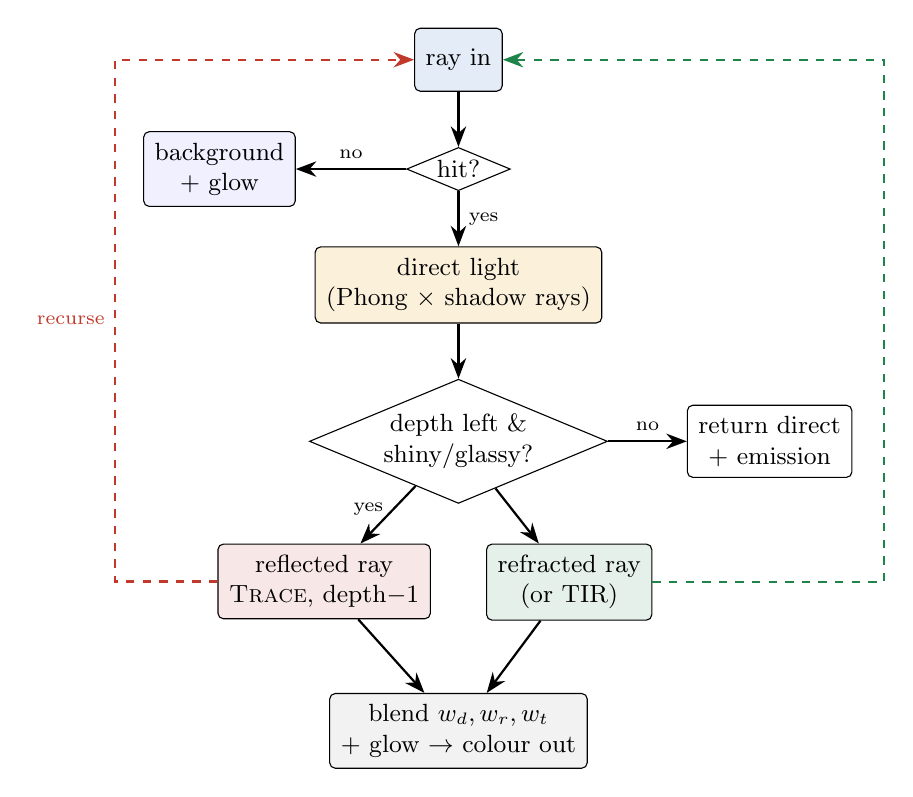
\begin{tikzpicture}[node distance=7mm and 9mm,
  box/.style={draw, rounded corners=2pt, align=center, font=\small, minimum height=8mm, inner sep=4pt, fill=white},
  dec/.style={draw, diamond, aspect=2.4, align=center, font=\small, inner sep=1pt, fill=white},
  flow/.style={->, thick}]
  \node[box, fill=cPrimary!12] (ray) {ray in};
  \node[dec, below=of ray] (hit) {hit?};
  \node[box, left=14mm of hit, fill=blue!6] (bg) {background\\+ glow};
  \node[box, below=of hit, fill=cLight!15] (dir) {direct light\\(Phong $\times$ shadow rays)};
  \node[dec, below=of dir] (more) {depth left \&\\shiny/glassy?};
  \node[box, right=10mm of more] (leaf) {return direct\\+ emission};
  \node[box, below left=9mm and -6mm of more, fill=cRefl!12] (refl) {reflected ray\\$\textsc{Trace}$, depth$-1$};
  \node[box, below right=9mm and -6mm of more, fill=cRefr!12] (refr) {refracted ray\\(or TIR)};
  \node[box, below=24mm of more, fill=black!5] (mix) {blend $w_d,w_r,w_t$\\+ glow $\to$ colour out};
  \draw[flow] (ray) -- (hit);
  \draw[flow] (hit) -- node[above, font=\scriptsize] {no} (bg);
  \draw[flow] (hit) -- node[right, font=\scriptsize] {yes} (dir);
  \draw[flow] (dir) -- (more);
  \draw[flow] (more) -- node[above, font=\scriptsize] {no} (leaf);
  \draw[flow] (more) -- node[left, font=\scriptsize, pos=0.4] {yes} (refl);
  \draw[flow] (more) -- (refr);
  \draw[flow] (refl) -- (mix);
  \draw[flow] (refr) -- (mix);
  \draw[flow, cRefl, dashed] (refl.west) -- ++(-1.3,0) |- node[pos=0.25, left, font=\scriptsize] {recurse} (ray.west);
  \draw[flow, cRefr, dashed] (refr.east) -- ($(refr.east -| leaf.east)+(0.4,0)$) |- (ray.east);
\end{tikzpicture}
\caption{Control flow of \textsc{Trace}. The dashed arrows are the recursive calls.}
\end{figure}

\appendix
%===================================================================
\section{Notes from reading the code}
%===================================================================

The sections above describe what each stage is \emph{meant} to do. While reading
the implementation, a few places stood out where the code seems to behave
differently. They are worth double-checking:

\begin{enumerate}[leftmargin=1.6em]
  \item \textbf{Refraction indices on entry/exit were swapped (fixed).}
        Previously, on \emph{entering} both $n_1$ and $n_2$ were set to the
        ray's current index, so $\eta=1$ and the ray passed into the object
        without bending. On \emph{leaving}, the pair was reversed, so the ray
        bent as if it were entering, and total internal reflection could never
        happen. The code now uses the pairing from Section~\ref{sec:refraction}
        (entering: $n_{\text{ray}}\to n_O$; leaving: $n_O\to n_{\text{surround}}$).
        A glass ball now inverts the scene behind it like a real lens, and TIR
        shows up inside glass (see \texttt{docs/refraction\_fix/}).
  \item \textbf{Directional-light shadow rays point away from the light.} The
        diffuse term treats the stored direction as pointing \emph{toward} the
        light ($\dotp{\vv N}{\vv L}$), and the origin offset picks the hemisphere
        with the same sign. The shadow ray, however, is shot along the
        \emph{negated} direction, and the brightness also uses the negated
        direction, so it is $\le 0$ (fully dark) on faces turned toward the
        light. Shooting the shadow ray along the stored direction and using
        $\dotp{\vv N}{\vv L}$ would match the point-light logic.
  \item \textbf{Schlick when leaving a dense medium.} For $n_1>n_2$, the
        approximation is more accurate with $\cos\theta_2$ (the transmitted
        angle) in place of $\cos\theta_1$. Otherwise $R_F$ stays low right up to
        the critical angle. Since TIR is handled separately, this is a
        quality issue rather than a bug.
  \item \textbf{Direct light on transparent surfaces is attenuated twice}: once
        by $(1-\tau)$ and once more by $w_d\approx1-\rho-\tau$. For $\tau=0.7$
        the direct term ends up weighted by about $0.09$. That may be intended
        (to keep glass clear), but one of the two factors is probably enough.
  \item \textbf{Emission is only added at leaves.} An emissive sphere that is
        also reflective or transparent goes down the recursive branch and loses
        its own emission (glow along the ray is still added).
\end{enumerate}

\end{document}
